\documentclass[a4paper]{article}
\usepackage[T5]{fontenc}
\usepackage[utf8]{inputenc}
% \usepackage{vntex}
\usepackage[english]{babel}
%\usepackage[utf8]{inputenc}
%\usepackage[francais]{babel}
\usepackage{geometry}
\geometry{
  a4paper,
  left=2.5cm,
  right=2.5cm,
  top=2.5cm,
  bottom=2.5cm
}
\usepackage{amssymb,epsfig,latexsym,multicol,array,hhline,fancyhdr}
\usepackage{booktabs}
\usepackage{amsmath}
\usepackage{lastpage}
\usepackage{comment}
\usepackage{enumitem}
\usepackage[lined,boxed,commentsnumbered]{algorithm2e}
\usepackage{enumerate}
\usepackage{color}
\usepackage{graphicx}							% Standard graphics package
\usepackage{array}
\usepackage{tabularx, caption}
\usepackage{multirow}
\usepackage{wrapfig,lipsum,booktabs}
\usepackage[framemethod=tikz]{mdframed}% For highlighting paragraph backgrounds
\usepackage{multicol}
\usepackage{rotating}
\usepackage{geometry}
\usepackage{setspace}
\usepackage{epsfig}
\usepackage{tikz}
\usetikzlibrary{shapes.geometric, arrows, positioning}
\usepackage{pgfplots}
\pgfplotsset{compat=1.18}
\usepackage{listings}
\usepackage{textcomp}
\usepackage{gensymb}
\usepackage{float}
% \usepackage[demo]{graphicx} % Removed to avoid option clash
\usepackage{hyperref}

\hypersetup{urlcolor=blue,linkcolor=black,citecolor=black,colorlinks=true}
%\usepackage{pstcol} 								% PSTricks with the standard color package

\newtheorem{theorem}{{\bf Theorem}}
\newtheorem{property}{{\bf Property}}
\newtheorem{proposition}{{\bf Proposition}}
\newtheorem{corollary}[proposition]{{\bf Corollary}}
\newtheorem{lemma}[proposition]{{\bf Lemma}}

\AtBeginDocument{\renewcommand*\contentsname{Contents}}
\AtBeginDocument{\renewcommand*\refname{References}}
\renewcommand*{\figurename}{Figure }

\newlength{\imageLength}
\setlength{\imageLength}{0.99\textwidth}
\setlength{\parindent}{0pt}

\NewDocumentCommand{\codeword}{v}{%
\texttt{\textcolor{blue}{#1}}%
}

% \everymath{\color{blue}}
%\usepackage{fancyhdr}
\setlength{\headheight}{40pt}
\pagestyle{fancy}
\fancyhead{} % clear all header fields
\fancyhead[L]{
 \begin{tabular}{rl}
    \begin{picture}(25,15)(0,0)
    \put(0,-8){\includegraphics[width=10mm, height=10mm]{graphics/HCMUT.png}}
    %\put(0,-8){
\epsfig{width=10mm,figure=hcmut.eps}}
   \end{picture}&
	%
\includegraphics[width=8mm, height=8mm]{hcmut.png} & %
	\begin{tabular}{l}
		\textbf{\bf \ttfamily HO CHI MINH CITY
UNIVERSITY OF TECHNOLOGY}\\
		\textbf{\bf \ttfamily FACULTY OF COMPUTER SCIENCE AND ENGINEERING}
	\end{tabular}
 \end{tabular}
}
\fancyhead[R]{
	\begin{tabular}{l}
		\tiny \bf \\
		\tiny \bf
	\end{tabular}  }
\fancyfoot{} % clear all footer fields
\fancyfoot[L]{\scriptsize \ttfamily Natural Language Processing (CO3086)}
\fancyfoot[R]{\scriptsize \ttfamily Page {\thepage}/\pageref{LastPage}}
\renewcommand{\headrulewidth}{0.3pt}
\renewcommand{\footrulewidth}{0.3pt}


%%%
\setcounter{secnumdepth}{4}
\setcounter{tocdepth}{3}
\makeatletter
\newcounter {subsubsubsection}[subsubsection]
\renewcommand\thesubsubsubsection{\thesubsubsection .\@alph\c@subsubsubsection}
\newcommand\subsubsubsection{\@startsection{subsubsubsection}{4}{\z@}%
                                     {-3.25ex\@plus -1ex \@minus -.2ex}%
                                     {1.5ex \@plus .2ex}%
                                     {\normalfont\normalsize\bfseries}}
\newcommand*\l@subsubsubsection{\@dottedtocline{3}{10.0em}{4.1em}}
\newcommand*{\subsubsubsectionmark}[1]{}
\makeatother

\definecolor{dkgreen}{rgb}{0,0.6,0}
\definecolor{gray}{rgb}{0.5,0.5,0.5}
\definecolor{mauve}{rgb}{0.58,0,0.82}

\lstset{frame=tb,
	language=Matlab,
	aboveskip=3mm,
	belowskip=3mm,
	showstringspaces=false,
	columns=flexible,
	basicstyle={\small\ttfamily},
	numbers=none,
	numberstyle=\tiny\color{gray},
	keywordstyle=\color{blue},
	commentstyle=\color{dkgreen},
	stringstyle=\color{mauve},
	breaklines=true,
	breakatwhitespace=true,
	tabsize=3,
	numbers=left,
	stepnumber=1,
	numbersep=1pt,
	firstnumber=1,
	numberfirstline=true
}

\begin{document}
%%%%%%%%%%%%%%%%%%%%%%%%%%%%%%%%%
\begin{titlepage}
\begin{center}
VIETNAM NATIONAL UNIVERSITY, HO CHI MINH CITY \\
UNIVERSITY OF TECHNOLOGY \\
FACULTY OF COMPUTER SCIENCE AND ENGINEERING
\end{center}

\vspace{1cm}

\begin{figure}[h!]
\begin{center}

\includegraphics[width=3cm]{graphics/hcmut.png}
\end{center}
\end{figure}

\vspace{0.8cm}

\begin{center}
\textbf{{\Large NATURAL LANGUAGE PROCESSING (CO3086)}}\\
\vspace{1.0cm}
\textbf{{\large ASSIGNMENT REPORT}}\\
\vspace{0.4cm}
\rule{\linewidth}{0.5pt}
\vspace{1.0cm}
{\LARGE\bfseries Analyzing and Comparing Text Preprocessing and\\[-1.0ex]
Tokenization Methods for Large-Scale Language Modeling\par}
\vspace{1.0cm}
\rule{\linewidth}{0.5pt}
\vspace{1.0cm}
\textbf{{\Large CC01 - Group 03}}\\
\end{center}

\vspace{0.5cm}

\begin{table}[h]
\centering
\begin{tabular}{rl}
\textbf{Advisors:}
& Ph.D Trương Vĩnh Lân \\
& Mr. Bùi Khánh Vĩnh \\
\textbf{Students:}
& Võ Hoàng Phúc - 2252650\\
& Vũ Minh Quân - 2212828\\
& Vũ Hoàng Tùng - 2252886\\
& Trần Đặng Hiển Long - 2252449\\
\end{tabular}
\end{table}

\begin{center}
{\footnotesize HO CHI MINH CITY, APRIL 2026}
\end{center}
\end{titlepage}

\thispagestyle{empty}
\newpage

%%%%%%%%%%%%%%%%%%%%%%%%%%%%%%%%%

%%%%%%%%%%%%%%%%%%%%%%%%%%%%%%%%%

\tableofcontents
\newpage
\section*{Work Assignment and Report Coverage}

\subsection*{Team Member Assignment}
\begin{table}[h!]
\centering
\renewcommand{\arraystretch}{1.2}
\begin{tabular}{|c|l|p{8.0cm}|c|}
\hline
\textbf{Student ID} & \textbf{Full Name} & \textbf{Mission} & \textbf{Completion} \\ \hline
2252449 & Trần Đặng Hiển Long & Experimental setup, preprocessing pipeline, and language-model evaluation. & 100\% \\ \hline
2212828 & Vũ Minh Quân & Consolidation of report materials and BPE knowledge synthesis& 100\% \\ \hline
2252650 & Võ Hoàng Phúc & Word-level and character-level tokenization write-up, and comparative analysis. & 100\% \\ \hline
2252886 & Vũ Hoàng Tùng & BPE theory, methodology, and interpretation of results in intrinsic and extrinsic evaluations. & 100\% \\ \hline
\end{tabular}
\caption{Team member task assignment}
\end{table}

\subsection*{Checklist Against Assignment Requirements}
\begin{itemize}
    \item \textbf{Overview of text preprocessing in NLP and its importance in language modeling:} Covered in Section 1.
    \item \textbf{Detailed explanation of word-level, character-level, and BPE-based tokenization methods:} Covered in Section 2.
    \item \textbf{Comparative analysis of vocabulary size, sequence length, and computational efficiency:} Covered in Section 3.
    \item \textbf{Experimental results on One Billion Word, WikiText-103, Text8, and Enwik8:} Covered in Section 4.
    \item \textbf{Impact on language modeling performance (e.g., perplexity and training speed):} Covered in Section 4.
    \item \textbf{Insights, limitations, and conclusions:} Covered in Section 5.
    \item \textbf{Implementation details for preprocessing, tokenization, and experiments:} Summarized in Section 4.
\end{itemize}

\subsection*{Source Code Repository}
The complete implementation of the preprocessing pipeline, tokenization methods, and language modeling experiments is available at the following repository:
\begin{center}
    \url{https://github.com/Iongshiba/nlp-assignment}
\end{center}

\newpage
\section{Introduction}

\subsection{Context and Motivation}
In simple terms, tokenization is the process of breaking text into smaller units, known as tokens. These tokens can be words, characters, sentences, or phrases, depending on the tokenization method used. In the development of Language Models (LMs), text preprocessing and tokenization serve as the critical interface between raw natural language data and deep learning architectures. More than just text cleaning and segmentation, it converts raw unstructured natural language into its numerical representation that computers can understand and perform statistical modeling, leading to the recent explosion of AI technologies. How we tokenize a corpus—that is, how we decide to represent our language numerically—dictates model embedding space distributions, memory complexity, and accuracy. As proven from modern benchmarks like One Billion Word or WikiText-103 representing large-scale corpora, a good tokenization strategy lays a foundational decision that impacts every subsequent stage of the pipeline.

\subsection{Problem Statement}
\label{token_probs}
Surveying the evolution of tokenization from its earliest forms, the paradigm has consistently struggled with two core technical limitations. First is the \textbf{Vocabulary Problem (Memory vs. Meaning)}. Intuitively, for a model to understand an entire corpus, it would need an enormous "dictionary" that captures every possible word and combination so each word has its own meaningful numeric representation. This costs vast amounts of memory. Even worse, the system still falls short in robustness as it encounters unseen words, leading to the well-known Out-of-Vocabulary (OOV) issue, where such inputs are treated as complete unknowns, causing semantic loss and discontinuity.

As another application-related limitation, the \textbf{Sequence Problem (Speed vs. Complexity)} emerges when we try to avoid the vocabulary explosion by decomposing text into smaller units. While this keeps the dictionary compact, it dramatically increases sequence length. Since modern architectures like Transformers scale poorly with longer sequences, both training and inference become significantly slower and more costly. On top of that, tokenization, like any other encoding method, inevitably introduces information loss: by treating sentences as a sequence of discrete numeric tokens, they may lose certain grammatical as well as semantic essences. 

Thus, research in tokenization fundamentally revolves around finding a "sweet spot"—a tokenization process that produces tokenizers compact enough to be efficient and memory-friendly, yet expressive enough to preserve meaning.

\subsection{Objective}
The objective of this assignment is to conduct an empirical study comparing different tokenization strategies. Specifically, the study aims to:
\begin{itemize}
    \item Implement and analyze three major tokenization paradigms: Word-level, Character-level, and Byte Pair Encoding (BPE).
    \item Evaluate the performance of these methods across diverse datasets including WikiText-103, One Billion Word, Text8, and Enwik8.
    \item Measure the impact of vocabulary size on compression ratios and sequence lengths.
    \item Observe how different tokenization choices affect downstream language modeling metrics such as training speed and perplexity.
\end{itemize}

\section{Text Preprocessing and Tokenization Methods}

\subsection{Preprocessing Pipeline}
Before tokenization, the corpora are normalized to reduce unnecessary variation that does not contribute useful linguistic signals for the planned experiments. The preprocessing pipeline includes lowercasing, normalization of quotation marks and dashes to ASCII-friendly forms, whitespace cleanup, and filtering of unsupported symbols using a fixed regular-expression policy. This preprocessing stage ensures that differences observed later are primarily attributable to the tokenization strategies themselves rather than inconsistent text formatting.

\subsection{Word-level Tokenization}
Word-level tokenization is the most intuitive approach, where each unique word in a corpus is translated into a single token for the model by being mapped to a discrete integer ID. Formally, this process is defined by a mapping function $f: S \rightarrow \{T_1, T_2, \dots, T_n\}$ where $S$ is the raw input string and each $T_i$ belongs to a predefined vocabulary $V$. For example, the sentence "Learning NLP is fun" is translated directly into \texttt{["Learning", "NLP", "is", "fun"]}.

\textbf{Advantages and Limitations:}
\begin{itemize}
    \item \textbf{Pros:} It preserves the clear semantic meaning of words, making the embedding space easier for the model to navigate. It also produces relatively short sequences.
    \item \textbf{Cons:} It suffers from Zipf's Law, leading to a massive vocabulary size. This creates the "Out-of-Vocabulary" (OOV) problem, where rare words are mapped to a lossy \texttt{<UNK>} token, causing semantic loss.
\end{itemize}

\subsection{Character-level Tokenization}
This method breaks text down into the most atomic units: individual letters and symbols. If $S$ is the input sentence and $C$ is its character-level representation, it typically holds that $|C| \gg |S|$, significantly increasing the sequence length. For example, "NLP" is decomposed into \texttt{["N", "L", "P"]}.

\textbf{Advantages and Limitations:}
\begin{itemize}
    \item \textbf{Pros:} It results in an extremely small vocabulary (usually $|V| < 300$) and effectively has a 0\% OOV rate, as any word can be built from characters.
    \item \textbf{Cons:} It produces much longer sequences, increasing the computational burden on the model's attention or recurrence mechanisms. It also forces the model to learn meaning from "scratch" without inherent semantic cues.
\end{itemize}

\subsection{Byte Pair Encoding (BPE)}
BPE is a subword tokenization method serving as a hybrid between words and characters. It starts with a character-level base and iteratively merges the most frequent adjacent pairs until a target vocabulary size $K$ is reached. This allows the model to "see" relationships between related words (e.g., "play", "player", "played") by isolating shared roots.

\subsubsection{Study of Methodology: The BPE Mechanics}
Unlike Word-level tokenization, BPE is a bottom-up clustering process. To demonstrate its deterministic nature, consider a small corpus:
\begin{itemize}
    \item \textbf{Train:} "the player played a professional game", "the players are playing several games"
    \item \textbf{Vocabulary Learning:} BPE learns to group high-frequency patterns. The sequence \texttt{p+l+a+y} appears frequently, forming the token \texttt{play}. Suffixes like \texttt{ing} or words like \texttt{professional} are also merged.
    \item \textbf{Inference:} When applying these rules to "a professional plays the game", BPE recognizes \texttt{professional} and \texttt{play} as units. Even if "plays" wasn't in the train set, it can be decomposed into \texttt{[play, s]}, avoids the OOV issue.
\end{itemize}

\begin{table}[H]
\centering
\begin{tabular}{|l|c|c|c|}
\hline
\textbf{Feature} & \textbf{Word-level} & \textbf{Char-level} & \textbf{BPE} \\ \hline
Vocab Size & 9 unique words & 14 unique chars & Optimized $K$ \\ \hline
Sequence Length & 4 tokens + \texttt{<UNK>} & 32 characters & 5 subwords \\ \hline
\end{tabular}
\caption{Comparative metrics on a controlled long-sentence corpus}
\label{tab:bpe_long_comp}
\end{table}

BPE serves as a "sweet spot": it breaks words into core components to ensure no information is lost while avoiding the excessive sequence lengths of character tokenization.

\section{Comparative Analysis of Tokenization Strategies}
A comprehensive comparative analysis of the proposed tokenization methods—Word-level, Character-level, and Byte Pair Encoding (BPE)—is conducted based on three critical criteria. This analysis evaluates the inherent trade-offs each method presents and how they ultimately dictate the architectural design of language models.

\begin{itemize}
    \item \textbf{Vocabulary Size}: Impact on memory footprint, embedding matrix dimensionality, and semantic coverage.
    \item \textbf{Sequence Length}: Impact on information compression, context window limitations, and long-term dependency tracking.
    \item \textbf{Computational Efficiency}: Impact on temporal processing bottlenecks, training speed, and inference latency.
\end{itemize}

\subsection{Vocabulary Size and Memory Footprint}
The size of the vocabulary ($|V|$) directly dictates the dimensions of the model's first and last layers: the input embedding matrix and the final output projection layer (softmax). A larger vocabulary exponentially increases the total trainable parameters of the model.

\begin{itemize}
    \item \textbf{Word-level Tokenization:} This method inherently suffers from the sparse, long-tail distribution of natural language, dictated by Zipf's Law. To maintain an acceptable Out-of-Vocabulary (OOV) rate, the model requires an excessively large dictionary (often exceeding 50,000 to 100,000 tokens). This heavily inflates the embedding layer, consuming massive amounts of GPU memory. Furthermore, the representations of rare words in the long tail suffer from extreme sparsity; because they appear infrequently during training, their embeddings are rarely updated, leading to poor generalization and a high risk of overfitting.
    \item \textbf{Character-level Tokenization:} In stark contrast, character-level methods utilize a radically constrained and closed vocabulary (typically between 30 to 100 tokens, encompassing standard alphabets, digits, and essential punctuation). This approach completely eliminates the OOV problem. Consequently, it shrinks the embedding matrix to a negligible size, drastically reducing the model's structural memory footprint and parameter count, making it highly suitable for strictly memory-constrained environments.
    \item \textbf{BPE-based Tokenization:} Byte Pair Encoding (BPE) offers an elegant, data-driven mathematical compromise. By establishing a user-defined target vocabulary size (e.g., 30,000 to 50,000), BPE maintains a bounded memory footprint. Because it dynamically merges characters into subwords based on corpus frequency, it completely bypasses the OOV issue by breaking down unknown or rare words into familiar subword units. This ensures that the embedding matrix is populated entirely by dense, frequently updated representations rather than sparse rare words.
\end{itemize}

\subsection{Sequence Length and Context Window}
Sequence length determines the temporal dimension of the input data. It dictates how effectively a sequence model (such as an LSTM or Transformer) can capture long-term semantic dependencies within a fixed computational context window.

\begin{itemize}
    \item \textbf{Word-level Tokenization:} Provides the highest text compression ratio (often compressing characters down to $\sim$17-20\% of their original count). Because an entire semantic concept (a word) is represented by a single token, the average sequence length is extremely short. This allows recurrent models to easily capture long-term semantic context spanning across multiple sentences without encountering severe vanishing gradient issues over time.
    \item \textbf{Character-level Tokenization:} Exhibits the absolute poorest compression ratio (strictly 1.0). A single sentence must be decomposed into dozens, or even hundreds, of individual character tokens. Consequently, sequence lengths inflate drastically (typically 400\% to 600\% longer than word-level representations). This places an immense burden on the model's context window. During training, the Backpropagation Through Time (BPTT) algorithm must traverse a massively long computational graph, making it exceedingly difficult for the network to remember dependencies from the beginning of a sentence due to the vanishing gradient problem.
    \item \textbf{BPE-based Tokenization:} Achieves an optimal, intermediate sequence length. Highly frequent words (like "the", "is", "apple") remain unified as single tokens—behaving exactly like word-level tokenization. Conversely, only rare or complex morphological words are fractured into subwords (e.g., "un-break-able"). The resulting overall sequence length is only marginally longer than a pure word-level approach, but vastly shorter and much more manageable than a character-level sequence.
\end{itemize}

\subsection{Computational Efficiency}
Efficiency is evaluated by analyzing the primary mathematical bottlenecks during the forward and backward passes, specifically focusing on sequential unrolling (temporal steps) and the final probability distribution calculation (softmax).

\begin{itemize}
    \item \textbf{Word-level Tokenization:} While temporal processing is remarkably fast due to the short sequence lengths, the computational bottleneck abruptly shifts to the final layer. Calculating the softmax probabilities over a massive vocabulary of 50,000+ tokens at every single timestep requires massive matrix multiplications. This is highly computationally expensive, drastically slowing down both training throughput and real-time inference latency.
    \item \textbf{Character-level Tokenization:} The softmax calculation is exceptionally cheap and lightning-fast due to the microscopic vocabulary size (e.g., 52 tokens). However, the sheer volume of sequential timesteps creates a severe temporal bottleneck. Because recurrent models process data sequentially, unrolling an LSTM for 1,000 character steps takes significantly longer than unrolling it for 200 word steps. This causes the training time per epoch to skyrocket, nullifying the speed gained from the small softmax layer.
    \item \textbf{BPE-based Tokenization:} BPE strikes the ultimate architectural balance for modern language models. The vocabulary size is sufficiently constrained to prevent the softmax calculation from becoming a severe bottleneck, while the sequence length remains compact enough to ensure extremely fast temporal processing. Furthermore, because subwords carry intrinsic morphological meaning (unlike standalone characters that lack independent semantic value), the model converges much faster during training.
\end{itemize}

\subsection{Factors Affecting BPE Performance}
Based on the empirical study by V\~u Ho\`ang T\`ung, the effectiveness of BPE is primarily dictated by two factors: the vocabulary budget $K$ and the entropy of the training data.

\begin{itemize}
    \item \textbf{Vocabulary Budget ($K$):} The choice of $K$ is the most critical factor. If $K$ is too low, common words may remain fragmented (e.g., \texttt{[pro, fess, ion, al]}), increasing sequence lengths and computational steps. Conversely, if $K$ is too high, the tokenizer may merge words into rare symbols that appear only once, wasting the vocabulary budget and increasing memory costs in the embedding layer ($|V| \times d$).
    \item \textbf{Data Entropy:} BPE performance is heavily tied to the regularity of the training data. In structured datasets like \textit{WikiText-103}, frequent English morphemes allow for high reuse of merge rules. In contrast, high-entropy or noisy data like \textit{Enwik8} leads to fragmentation where merge rules are less "universal," potentially wasting the vocabulary budget.
\end{itemize}

\subsection{BPE as the "Sweet Spot"}
The comparative evidence suggests that BPE acts as a practical "sweet spot" between the two extremes. Relative to word-level tokenization, it sacrifices only a small amount of compression while removing OOV failures. Relative to character-level tokenization, it preserves lexical coverage without exploding sequence length. This makes it the most robust choice for open-domain language modeling where both efficiency and coverage are paramount.

\section{Experimental Setup and Results}

\subsection{Experimental Setup}
This section follows the experimental configuration consolidated by Trần Đặng Hiển Long and uses it as the authoritative setup for the final report. The study evaluates three tokenization strategies---word-level, character-level, and BPE---on four benchmark corpora.

\subsubsection{Preprocessing Pipeline}
\begin{figure}[H]
    \centering
    \begin{tikzpicture}[node distance=1.5cm, every node/.style={fill=white, font=\footnotesize}, align=center]
        \node (raw) [draw, rectangle] {Raw Text \\ (e.g., WikiText-103)};
        \node (norm) [draw, rectangle, below of=raw] {Normalization \\ (Lowercasing, Smart Quotes $\rightarrow$ ASCII)};
        \node (clean) [draw, rectangle, below of=norm] {Character Filtering \\ (Regex Policy)};
        \node (chunk) [draw, rectangle, below of=clean] {Chunking \\ (Text8: 200w / Enwik8: 1000ch)};
        \node (token) [draw, diamond, aspect=2, below of=chunk, node distance=2cm] {Tokenization Type?};
        
        \draw [->] (raw) -- (norm);
        \draw [->] (norm) -- (clean);
        \draw [->] (clean) -- (chunk);
        \draw [->] (chunk) -- (token);
        
        \node (word) [draw, rectangle, below left of=token, node distance=2.5cm, xshift=-1cm] {Word-level};
        \node (char) [draw, rectangle, below of=token, node distance=2.5cm] {Character-level};
        \node (bpe) [draw, rectangle, below right of=token, node distance=2.5cm, xshift=1cm] {BPE (Subword)};
        
        \draw [->] (token) -| (word);
        \draw [->] (token) -- (char);
        \draw [->] (token) -| (bpe);
    \end{tikzpicture}
    \caption{Preprocessing and Tokenization Flowchart}
    \label{fig:pipeline_flow}
\end{figure}

The preprocessing pipeline uses a fixed random seed of 42. Before tokenization, text is lowercased, tabs and line breaks are normalized, and repeated whitespace is collapsed. A strict character-filtering regular expression is applied to keep only alphanumeric symbols, spaces, and a selected punctuation subset: \texttt{[a-z0-9\textbackslash s\textbackslash .\textbackslash ,!\textbackslash ?;:'"\textbackslash -\textbackslash (\textbackslash )]}.

\subsubsection{Datasets and Chunking}
Existing train/validation/test splits are reused for \textit{One Billion Word} and \textit{WikiText-103}. For \textit{Text8} and \textit{Enwik8}, the data is shuffled and split into 90\% train, 5\% validation, and 5\% test. To manage sequence geometry during training, \textit{Text8} is chunked into 200-word segments, while \textit{Enwik8} uses segments of 1000 characters.

\subsubsection{Tokenizer Configuration}
All tokenizers share the special tokens \texttt{<PAD>}, \texttt{<UNK>}, \texttt{<BOS>}, and \texttt{<EOS>}.
\begin{itemize}
    \item \textbf{Word-level:} Regex-based segmentation with a target vocabulary sweep.
    \item \textbf{Character-level:} Character-set vocabulary derived from the training corpus.
    \item \textbf{BPE:} Implemented via the Hugging Face \texttt{tokenizers} library with a \texttt{Whitespace()} pre-tokenizer.
\end{itemize}

\subsubsection{Language Modeling Configuration}
To examine downstream effects, we train an LSTM-based language model with the following shared hyperparameters: embedding size 128, hidden size 256, 2 layers, batch size 32, sequence length 128, learning rate 0.001, and random seed 42. Perplexity and avg. epoch time are calculated across a fixed budget of 3--5 epochs depending on the comparison.

\subsection{Tokenization Evaluation}
The performance metrics for each tokenizer are summarized across multiple configurations. The data reveals a clear inverse relationship between the vocabulary size and the resulting average sequence length ($L_{avg}$), alongside the critical trade-off with the Out-of-Vocabulary (OOV) rate.

\begin{table}[h]
\centering
\caption{Consolidated Benchmarks: OOV Penalties vs. Optimized Subword Compression}
\label{tab:final_relative_results}
\resizebox{\textwidth}{!}{
\begin{tabular}{|l|l|r|l|r|l|}
\hline
\textbf{Dataset} & \textbf{Tokenizer} & \textbf{Vocab} & \textbf{Avg. Seq. Len} $\downarrow$ & \textbf{OOV (\%)} $\uparrow$ & \textbf{Comp. Ratio} $\downarrow$ \\ \hline
\multirow{7}{*}{\textbf{Text8}} & Char & 31 & 1178.08 (+489.0\%) & 0.00\% & 1.00 (+489.0\%) \\ \cline{2-6}
 & BPE-2k & 2,000 & 318.36 (+59.2\%) & 0.00\% & 0.27 (+59.2\%) \\ \cline{2-6}
 & BPE-8k & 8,000 & 247.50 (+23.8\%) & 0.00\% & 0.21 (+23.8\%) \\ \cline{2-6}
 & BPE-16k & 16,000 & 226.54 (+13.3\%) & 0.00\% & 0.19 (+13.3\%) \\ \cline{2-6}
 & BPE-32k & 32,000 & 213.80 (+6.9\%) & 0.00\% & 0.18 (+6.9\%) \\ \cline{2-6}
 & BPE-50k & 50,000 & 208.95 \underline{\textbf{(+4.5\%)}} & 0.00\% & 0.18 \underline{\textbf{(+4.5\%)}} \\ \cline{2-6}
 & Word & 50,000 & \textbf{200.00} & \textbf{2.77\%} & \textbf{0.17} \\ \hline \hline
\multirow{7}{*}{\textbf{Wiki-103}} & Char & 52 & 431.72 (+421.3\%) & 0.00\% & 1.00 (+421.3\%) \\ \cline{2-6}
 & BPE-2k & 2,000 & 125.78 (+51.9\%) & 0.00\% & 0.29 (+51.9\%) \\ \cline{2-6}
 & BPE-8k & 8,000 & 99.86 (+20.6\%) & 0.00\% & 0.23 (+20.6\%) \\ \cline{2-6}
 & BPE-16k & 16,000 & 92.65 (+11.9\%) & 0.00\% & 0.21 (+11.9\%) \\ \cline{2-6}
 & BPE-32k & 32,000 & 88.53 (+6.9\%) & 0.00\% & 0.21 (+6.9\%) \\ \cline{2-6}
 & BPE-50k & 50,000 & 86.82 \underline{\textbf{(+4.8\%)}} & 0.00\% & 0.20 \underline{\textbf{(+4.8\%)}} \\ \cline{2-6}
 & Word & 45,379 & \textbf{82.82} & \textbf{3.42\%} & \textbf{0.19} \\ \hline \hline
\multirow{7}{*}{\textbf{One Billion}} & Char & 52 & 135.27 (+408.2\%) & 0.00\% & 1.00 (+408.2\%) \\ \cline{2-6}
 & BPE-2k & 2,000 & 39.08 (+46.8\%) & 0.00\% & 0.29 (+46.8\%) \\ \cline{2-6}
 & BPE-8k & 8,000 & 30.95 (+16.3\%) & 0.00\% & 0.23 (+16.3\%) \\ \cline{2-6}
 & BPE-16k & 16,000 & 28.98 (+8.9\%) & 0.00\% & 0.21 (+8.9\%) \\ \cline{2-6}
 & BPE-32k & 32,000 & 28.03 (+5.3\%) & 0.00\% & 0.21 (+5.3\%) \\ \cline{2-6}
 & BPE-50k & 38,379 & 27.83 \underline{\textbf{(+4.5\%)}} & 0.00\% & 0.21 \underline{\textbf{(+4.5\%)}} \\ \cline{2-6}
 & Word & 29,164 & \textbf{26.62} & \textbf{3.83\%} & \textbf{0.20} \\ \hline \hline
\multirow{7}{*}{\textbf{Enwik8}} & Char & 52 & 925.72 (+377.2\%) & 0.00\% & 1.00 (+377.2\%) \\ \cline{2-6}
 & BPE-2k & 2,000 & 290.28 (+49.6\%) & 0.00\% & 0.31 (+49.6\%) \\ \cline{2-6}
 & BPE-8k & 8,000 & 231.30 (+19.2\%) & 0.00\% & 0.25 (+19.2\%) \\ \cline{2-6}
 & BPE-16k & 16,000 & 213.33 (+10.0\%) & 0.00\% & 0.23 (+10.0\%) \\ \cline{2-6}
 & BPE-32k & 32,000 & 201.98 (+4.1\%) & 0.00\% & 0.22 (+4.1\%) \\ \cline{2-6}
 & BPE-50k & 50,000 & 197.24 \underline{\textbf{(+1.7\%)}} & 0.00\% & 0.218 \underline{\textbf{(+2.2\%)}} \\ \cline{2-6}
 & Word & 50,000 & \textbf{194.00} & \textbf{3.41\%} & \textbf{0.213} \\ \hline
\end{tabular}
}
\end{table}

Our results confirm that BPE effectively serves as a "sweet spot" in the tokenization landscape. Although Word-level tokenization provides the theoretical baseline for compression (highlighted in \textbf{bold} in Table~\ref{tab:final_relative_results}), it consistently fails due to high OOV rates.

\subsubsection{Detailed Word-level Tokenization Results}
To investigate the vocabulary bottleneck, we evaluated word-level tokenization across three vocabulary scales (5,000, 10,000, and 50,000 tokens).

\begin{table}[H]
\centering
\caption{Word-level Tokenization Results (Scaling Effects)}
\renewcommand{\arraystretch}{1.1}
\begin{tabular}{|l|c|c|c|c|c|}
\hline
\textbf{Vocab Size} & \textbf{Split} & \textbf{Enwik8} & \textbf{One Billion} & \textbf{Text8} & \textbf{WikiText-103} \\ \hline
\multirow{2}{*}{5,000} & OOV (\%) & 15.55 & 11.72 & 16.18 & 14.84 \\ \cline{2-6}
& Comp. Ratio & 0.209 & 0.196 & 0.170 & 0.189 \\ \hline
\multirow{2}{*}{10,000} & OOV (\%) & 10.43 & 6.85 & 10.37 & 9.65 \\ \cline{2-6}
& Comp. Ratio & 0.209 & 0.196 & 0.169 & 0.189 \\ \hline
\multirow{2}{*}{50,000} & OOV (\%) & \textbf{3.41} & \textbf{1.31} & \textbf{2.77} & \textbf{2.76} \\ \cline{2-6}
& Comp. Ratio & 0.209 & 0.196 & 0.169 & 0.189 \\ \hline
\end{tabular}
\end{table}

\textbf{Insights from Word-level Sweeps:}
\begin{itemize}
    \item \textbf{Vocab 5k:} A 5,000-word limit causes severe semantic loss, with OOV rates spiking to $\sim$16\% on Text8 and Enwik8.
    \item \textbf{Vocab 10k:} Doubling the vocabulary size roughly halves the OOV rate on the One Billion Word dataset, yet $\sim$10\% OOV on other benchmarks remains problematic.
    \item \textbf{Vocab 50k:} At 50,000 tokens, the tokenizer achieves acceptable semantic retention (OOV $\le$ 3.4\%) and maintains high compression efficiency (0.16--0.20), though it still cannot reach the 0\% OOV threshold required for total robustness.
\end{itemize}

\subsubsection{Character-level Tokenization Results}
Character-level tokenization treats every individual character as a distinct token, completely eliminating OOV at the cost of extreme sequence inflation.

\begin{table}[H]
\centering
\caption{Character-level Tokenization Results}
\renewcommand{\arraystretch}{1.1}
\begin{tabular}{|l|c|c|c|c|}
\hline
\textbf{Metric (Test Split)} & \textbf{Enwik8} & \textbf{One Billion} & \textbf{Text8} & \textbf{WikiText-103} \\ \hline
\textbf{Absolute Vocab Size} & \textbf{52} & \textbf{52} & \textbf{31} & \textbf{52} \\ \hline
Avg Seq Length & 925.72 & 135.27 & 1178.08 & 431.72 \\ \hline
OOV Rate (\%) & 0 & 0 & 0 & 0 \\ \hline
Compression Ratio & 1.000 & 1.000 & 1.000 & 1.000 \\ \hline
\end{tabular}
\end{table}

\textbf{Insights from Character-level Trials:}
\begin{itemize}
    \item \textbf{Microscopic Vocabulary:} Uses only 31--52 tokens, drastically reducing the embedding memory footprint.
    \item \textbf{Sequence Inflation:} Sequence lengths explode (e.g., $\sim$1178 on Text8), placing an immense computational burden on recurrent models and hindering long-term context capture.
\end{itemize}

\subsubsection{BPE Results and Vocabulary Scaling}
BPE serves as the optimal bridge, providing complete OOV elimination while maintaining compression ratios near those of word-level models.

\begin{figure}[H]
    \centering
    \begin{tikzpicture}
    \begin{axis}[
        title={BPE Compression Scaling (One Billion Dataset)},
        xlabel={Vocabulary Size ($K$)},
        ylabel={Compression Ratio},
        xmin=0, xmax=55000,
        ymin=0.15, ymax=0.35, 
        xtick={0, 10000, 20000, 30000, 40000, 50000},
        ytick={0, 0.20, 0.25, 0.30, 0.35},
        scaled x ticks=false,
        xticklabel style={
            /pgf/number format/fixed,
            /pgf/number format/1000 sep={,}
        },
        % ------------------------------------------
        legend pos=north east,
        ymajorgrids=true,
        grid style=dashed,
        width=0.85\textwidth,
        height=7cm,
    ]

    % BPE Compression Curve
    \addplot[
        color=orange,
        mark=triangle*,
        line width=1pt,
        ]
        coordinates {
        (2000, 0.2889)(8000, 0.2288)(16000, 0.2143)(32000, 0.2073)(50000, 0.20573)
        };
        \addlegendentry{BPE Compression}

    % Word-level Baseline Ratio
    \addplot[
        color=red,
        dashed,
        line width=1pt,
        domain=0:50000,
    ] {0.1968};
    \addlegendentry{Word Baseline (0.197)}

    % Saturation Point Label
    \node[anchor=south west] at (axis cs:45000, 0.20573) {\small Saturation};

    \end{axis}
    \end{tikzpicture}
    \caption{BPE Compression Ratio correlation with K = 2k, 4k, 8k, 16k, 32k, 50k. The graph illustrates how BPE approaches the theoretical maximum density of Word-level tokenization without the cost of OOV errors.}
    \label{fig:compression_one_billion}
\end{figure}

Diving into the results from varying $K$ shown in Figure~\ref{fig:compression_one_billion}, we see a classic "elbow" pattern in the relationship between $K$ and $L_{avg}$. Increasing $K$ from 2,000 to 8,000 yields a substantial reduction in sequence length across all benchmarks. However, further increasing $K$ from 32,000 to 50,000 results in marginal efficiency gains. This observation justifies the common practice in modern LLMs of setting the vocabulary budget around 32k--50k. Beyond this threshold, the linear growth in memory cost for the embedding matrix and the computational overhead of the output Softmax layer outweigh the negligible gains in sequence compression.

\subsection{Evaluation of Language Model Performance}
The downstream impact of tokenization is evaluated by training LSTM-based language models across different corpora and vocabulary configurations.

\subsubsection{BPE Impact on Language Model Performance}
The training dynamics across the two most complex benchmarks, \textit{One Billion Word} and \textit{WikiText-103}, reveal several key insights into the synergy between BPE and language modeling.

\begin{table}[H]
\centering
\caption{LSTM Training Dynamics with BPE-36k Tokenization.}
\label{tab:lm_results}
\begin{tabular}{|l|c|c|c|c|}
\hline
\textbf{Dataset} & \textbf{Final Train PPL} & \textbf{Final Val PPL} & \textbf{Avg. Epoch Time (s)} & \textbf{Final BPC} \\ \hline
One Billion Word & 996.18 & 1145.49 & 7.90 & 1.3524* \\ \hline
WikiText-103     & 662.68 & 759.99  & 24.71 & 1.2841* \\ \hline
\end{tabular}
\end{table}

While the validation perplexity on \textit{WikiText-103} exhibited a sharp reduction (1521.50 $\rightarrow$ 759.99) over five epochs (or three in the unified setup), the convergence on \textit{One Billion Word} was markedly slower. Furthermore, a significantly higher training throughput was observed in lower-entropy corpora, reflecting BPE's adaptive compression.

\begin{figure}[H]
    \centering
    \begin{tikzpicture}
    \begin{axis}[
        title={Validation Perplexity Comparison (WikiText-103)},
        xlabel={Epoch},
        ylabel={Perplexity},
        xmin=1, xmax=5,
        ymin=500, ymax=1600,
        xtick={1,2,3,4,5},
        ytick={600, 800, 1000, 1200, 1400, 1600},
        legend pos=north east,
        ymajorgrids=true,
        grid style=dashed,
        width=0.85\textwidth,
        height=7cm,
    ]

    % K=16,000 Trend
    \addplot[
        color=blue,
        mark=square,
        line width=1pt,
        ]
        coordinates {
        (1, 1290.46)(2, 904.46)(3, 753.66)(4, 638.25)(5, 556.34)
        };
        \addlegendentry{BPE-16k}

    % K=36,000 Trend
    \addplot[
        color=red,
        mark=triangle,
        line width=1pt,
        ]
        coordinates {
        (1, 1521.50)(2, 1376.46)(3, 1011.68)(4, 863.56)(5, 759.99)
        };
        \addlegendentry{BPE-36k}

    \end{axis}
    \end{tikzpicture}
    \caption{Evolution of Validation Perplexity over 5 epochs for different vocabulary sizes.}
    \label{fig:ppl_k_comparison}
\end{figure}

The comparison between different vocabulary budgets on the WikiText-103 dataset reveals an interesting counter-intuitive result:
\begin{itemize}
    \item \textbf{Convergence Rate:} Contrary to the expectation that a larger vocabulary ($K=36k$) would facilitate better learning, the $K=16k$ configuration achieved a significantly lower final validation perplexity. This suggests that for a model of this scale (LSTM with 256 hidden units), a smaller, more dense vocabulary allows the model to learn token representations more effectively, as the parameter space for the embedding layer is smaller and easier to optimize.
    \item \textbf{Training Throughput:} There is a notable difference in computational cost. The $K=16k$ model trained significantly faster than the $K=36k$ model. This overhead is due to the larger Softmax layer at the output, which must compute probabilities over a wider range of tokens.
    \item \textbf{Information Bottleneck:} The higher perplexity of BPE-36k indicates that with a limited hidden size, increasing $K$ too much may lead to "sparsity" in token occurrences during training. The $K=16k$ model benefits from seeing each subword unit more frequently.
\end{itemize}

\subsubsection{Analysis of Tokenizers Impact on Language Model Performance}
To further examine the trade-offs across all tokenization families, we focus on five representative Enwik8 runs to compare perplexity and training speed under a fixed 3-epoch budget.

\begin{table}[H]
\centering
\caption{Enwik8 LM Results by Tokenizer Run (3 Epochs)}
\renewcommand{\arraystretch}{1.1}
\begin{tabular}{|l|c|c|c|}
\hline
\textbf{Tokenizer Run} & \textbf{Effective Vocab} & \textbf{Final Validation PPL} & \textbf{Avg Epoch Time (s)} \\ \hline
word\_2000 & 2000 & 20.853 & 107.805 \\ \hline
word\_36000 & 36000 & 91.595 & 247.414 \\ \hline
bpe\_2000 & 2000 & 53.018 & 540.036 \\ \hline
bpe\_36000 & 36000 & 178.612 & 255.976 \\ \hline
char\_2000 & 52 & 3.786 & 345.279 \\ \hline
\end{tabular}
\end{table}

\textbf{Perplexity and Speed Analysis:}
\begin{itemize}
    \item \textbf{Best Perplexity:} The character-level model obtains the lowest validation perplexity (3.786). However, this is achieved at a significant computational cost (345 s/epoch) due to sequence length.
    \item \textbf{Best Speed:} \texttt{word\_2000} is the fastest (107 s/epoch). Increasing the word vocabulary to 36k degrades both speed and perplexity, likely due to optimization sparsity.
    \item \textbf{BPE Scalability:} In BPE, increasing the vocabulary from 2k to 36k significantly improves speed (540s $\rightarrow$ 255s) because it shortens the sequences, though perplexity increases slightly under this fixed-epoch budget.
\end{itemize}

Under this specific configuration, \texttt{word\_2000} provides a strong speed-quality trade-off, while \texttt{char\_2000} minimizes perplexity at the cost of training time. BPE remains the most scalable solution for larger budgets and open-vocabulary scenarios.

\section{Discussion and Conclusion}

\subsection{Insights and Limitations}
The experiments confirm that tokenization is not an isolated preprocessing choice. It shapes the vocabulary space, sequence geometry, and optimization behavior of the downstream language model.

\begin{itemize}
    \item \textbf{Word-level tokenization} remains attractive when short sequences are the top priority, but its residual OOV rate limits robustness on realistic corpora.
    \item \textbf{Character-level tokenization} guarantees lexical coverage, yet its long sequences introduce a major computational burden and make modeling long-range dependencies harder.
    \item \textbf{BPE} consistently provides the strongest balance. It preserves near-word-level compression while retaining the ability to decompose rare words and remove OOV failures.
\end{itemize}

However, extrinsic evaluation reveals that linguistic efficiency does not always translate to better modeling performance. A critical \textbf{optimization bottleneck} was observed when scaling the vocabulary size. While a larger $K$ provides better sequence compression and captures more semantics per token, the resulting sparsity in the embedding space can halt gradient-based convergence. For our specific LSTM architecture, a smaller vocabulary allowed the model to calculate optimization momentum more effectively due to higher update frequency per token, leading to faster absolute convergence in a limited training budget.

The study has several limitations. The language-model experiments were conducted with a relatively small LSTM and a fixed training budget, so the conclusions about optimal vocabulary size are architecture-dependent. In addition, perplexity values across different tokenization families are not perfectly comparable because the prediction units themselves differ. Therefore, perplexity must be interpreted together with sequence length, coverage, and throughput.

\subsection{Conclusion}
This report studied text preprocessing and tokenization for large-scale language modeling through both theoretical analysis and empirical evaluation. On the four benchmark datasets---One Billion Word, WikiText-103, Text8, and Enwik8---the results show a consistent trade-off:
\begin{itemize}
    \item Word-level tokenization offers strong compression but suffers from OOV limitations;
    \item Character-level tokenization offers complete coverage but incurs severe sequence inflation;
    \item BPE best balances lexical coverage, compression, and computational efficiency.
\end{itemize}

The results validate BPE as the de facto tokenization strategy for modern NLP pipelines. It effectively eliminates the "information-computation" bottleneck, achieving proximity to word-level density while maintaining absolute lexical coverage.

\subsection{Recommendations}
This report studied text preprocessing and tokenization for large-scale language modeling through theoretical analysis and empirical evaluation. On the four benchmark datasets---One Billion Word, WikiText-103, Text8, and Enwik8---the results show a consistent trade-off:
\begin{itemize}
    \item \textbf{Word-level tokenization} offers strong compression but suffers from OOV limitations; it remains computationally attractive for training speed when the domain is strictly limited.
    \item \textbf{Character-level tokenization} offers complete coverage and minimizes token-level perplexity in current runs, but incurs severe sequence inflation and training costs.
    \item \textbf{BPE} best balances lexical coverage, compression, and computational efficiency, removing the OOV penalty while approaching word-level throughput.
\end{itemize}

As the final recommendation, the selection of an optimal tokenizer should depend on whether the specific application prioritizes training speed, lexical robustness, or semantic resolution. For general-purpose large-scale language modeling, BPE with a vocabulary budget in the range of 30,000 to 50,000 tokens provides the most robust and scalable trade-off. Future work can extend the study by testing transformer-based language models, broader multi-lingual datasets, and more complex token-level optimization strategies.


%%%%%%%%%%%%%%%%%%%%%%%%%%%%%%%%%
% \bibliographystyle{ieeetr}
%\bibliographystyle{ACM-Reference-Format-Journals}
\bibliographystyle{ieeetr}
\nocite{*}
\bibliography{ref}
\end{document}
